\chapter{Inicialización y Planificación}

\section{Identificación de Requerimientos}

\begin{table}[H]
    \caption{Título de la tabla}
    \label{tabla:ejemplo}
    \begin{center}
        \begin{tabular}{c|c|c|c|}
            \cline{2-4}
            & \textbf{Columna 1} & \textbf{Columna 2} & \textbf{Columna 3} \\ \hline
            \multicolumn{1}{|c|}{\textbf{Fila 1}} & item               & item               & item               \\ \hline
            \multicolumn{1}{|c|}{\textbf{Fila 2}} & item               & item               & item               \\ \hline
            \multicolumn{1}{|c|}{\textbf{Fila 3}} & item               & item               & item               \\ \hline
        \end{tabular}
    \end{center}
    Nota. Extraída de Apellido, N. (2000) \textit{Nombre del libro}.
    Editorial o universidad que lo publicó.
\end{table}

\section{Identificación de Subsistemas}
Referenciando a la figura \ref{fig:ejemplo}.
\begin{figure}[H]
    \begin{center}
        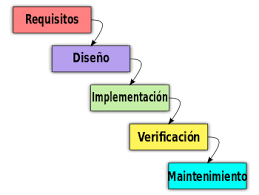
\includegraphics[width=6cm]{img/capitulo_4/cascada.png}
    \end{center}
    \caption{Ilustración de un ladrón}
    Fuente: Adaptada de Apellido, N. (2000) \textit{Nombre del libro}.
    Editorial o universidad que lo publicó.
    \label{fig:ejemplo}
\end{figure}

Referenciando a la figura \ref{fig:ejemplo}.
\begin{figure}[H]
    \begin{center}
        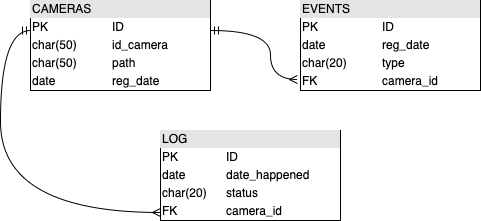
\includegraphics[width=10cm]{img/capitulo_4/db.png}
    \end{center}
    \caption{Ilustración de un ladrón}
    Fuente: Adaptada de Apellido, N. (2000) \textit{Nombre del libro}.
    Editorial o universidad que lo publicó.
    \label{fig:ejemplo}
\end{figure}

Referenciando a la figura \ref{fig:ejemplo}.
\begin{figure}[H]
    \begin{center}
        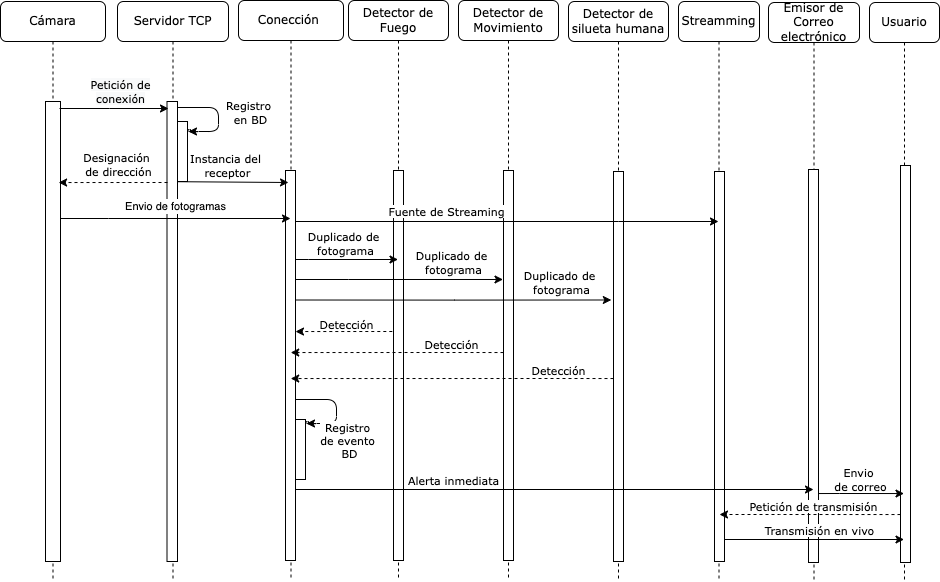
\includegraphics[width=18cm]{img/capitulo_4/interaccion.png}
    \end{center}
    \caption{Ilustración de un ladrón}
    Fuente: Adaptada de Apellido, N. (2000) \textit{Nombre del libro}.
    Editorial o universidad que lo publicó.
    \label{fig:ejemplo}
\end{figure}
\section{Comunicación de Sistemas}
\subsection{Sockets}

\subsection{ExoPlayer}

\section{Planificación}

